% Provenance (never printed): cycle 3 "Matiere, mouvement, energie,
% information" and "La planete Terre" (meteorological phenomena, the water in
% the air, measuring the weather); see sources/book1/PROVENANCE.md.
% Book 1, grade 4, chapter 1.
\chapter{Wolken, regen en sneeuw}\label{ch:g4:clouds-rain-snow}

Het is een warme zomermiddag. Rond het middageten was de lucht blauw, met
een paar kleine witte wolkjes als watjes. Om drie uur is een van die
wolkjes gegroeid. Hij zwelt op naar boven, hoger en hoger, als een witte
bloemkool op een platte grijze voet. Zijn top waaiert uit. Zijn onderkant
wordt donker. Er waait een koele windvlaag, de eerste dikke druppels vallen,
en twintig minuten lang giet het. Dan trekt de \omterm{def:g4:clouds-rain-snow:cloud}{wolk} weg, de zon komt terug
en de natte stoepen dampen.

Waar kwam die \omterm{def:g4:clouds-rain-snow:cloud}{wolk} vandaan? Waaruit bestaat hij? En hoeveel \omterm{def:g4:clouds-rain-snow:precipitation}{regen} is er in
die twintig minuten gevallen?

\begin{recall}
Het \omterm{def:g1:watching-the-weather:weather}{weer} is de toestand van de lucht op een bepaalde plek en een bepaald
moment: zonnig, bewolkt, \omterm{def:g4:clouds-rain-snow:precipitation}{regen}, \omterm{def:g4:clouds-rain-snow:precipitation}{sneeuw}, wind, \omterm{def:g4:clouds-rain-snow:cloud}{mist}; we schrijven het op in
een \omterm{def:g1:watching-the-weather:weather-chart}{weerkalender} (\cref{ch:g1:watching-the-weather}). Water uit de \omterm{def:g2:water-on-earth:ocean}{zee}, de
\omterm{def:g1:landscapes-around-us:water}{meren} en de grond stijgt op in de lucht en komt terug naar beneden als \omterm{def:g4:clouds-rain-snow:precipitation}{regen}
(\cref{ch:g2:water-on-earth}). De natuurkundeboeken vertellen hoe water
verdampt (van vloeistof naar een onzichtbaar gas), condenseert (van gas
terug naar piepkleine vloeistofdruppeltjes) en bevriest (van vloeistof naar
ijs), en hoe een thermometer de temperatuur meet in graden Celsius.
\end{recall}

\section{Wat is een wolk?}

De lucht om ons heen bevat altijd wat water, als een onzichtbaar gas:
waterdamp. Als lucht opstijgt, koelt ze af. Als ze genoeg afkoelt,
condenseert een deel van haar waterdamp tot waterdruppeltjes die zo klein
zijn dat het zwakste zuchtje wind ze laat zweven. Miljarden van die
druppeltjes naast elkaar vormen een \omterm{def:g4:clouds-rain-snow:cloud}{wolk} die we kunnen zien. Hoog in de
lucht, waar het heel koud is, bevriezen de druppeltjes en bestaat de \omterm{def:g4:clouds-rain-snow:cloud}{wolk}
uit piepkleine stukjes ijs.

\begin{definition}[Wolk en mist]\label{def:g4:clouds-rain-snow:cloud}
Een \emph{wolk}\index{wolk} is een enorm aantal piepkleine waterdruppeltjes,
of piepkleine stukjes ijs, die samen in de lucht zweven. \emph{Mist}\index{mist}
is een wolk die de grond raakt.
\end{definition}

\begin{example}[Je adem op een koude ochtend]\label{ex:g4:clouds-rain-snow:breath}
Op een koude ochtend maakt je adem een wit wolkje voor je mond. De lucht
die je uitademt is warm en bevat waterdamp. De koude lucht koelt haar
meteen af, de damp condenseert tot piepkleine druppeltjes --- en er
verschijnt een \omterm{def:g4:clouds-rain-snow:cloud}{wolk} in het klein, die weer verdwijnt als de druppeltjes
opnieuw verdampen.
\end{example}

Een \omterm{def:g4:clouds-rain-snow:cloud}{wolk} is wit omdat zijn druppeltjes het zonlicht alle kanten op
verstrooien. Als hij heel dik is, komt er weinig licht tot aan zijn
onderkant, en van onderaf ziet hij er grijs of bijna zwart uit: het teken
van een zware \omterm{def:g4:clouds-rain-snow:cloud}{wolk}, vol water.

\section{De wolkenfamilies}

\omterm{def:g4:clouds-rain-snow:cloud}{Wolken} hebben veel vormen, en weerwaarnemers over de hele wereld delen ze
op dezelfde manier in: naar hun vorm en naar hoe hoog ze zweven.

\begin{definition}[Wolkenfamilies]\label{def:g4:clouds-rain-snow:cloud-families}
De vier wolkenfamilies die je moet kennen, zijn:
\begin{itemize}
  \item \emph{cumulus}\index{cumulus}: stapelwolken, wit en bol, met een
        platte onderkant, als watjes;
  \item \emph{stratus}\index{stratus}: gelaagde \omterm{def:g4:clouds-rain-snow:cloud}{wolken}, een vlak grijs
        dek dat laag de hele hemel bedekt;
  \item \emph{cirrus}\index{cirrus}: vederwolken, dunne witte draden of
        krullen, heel hoog en van ijs;
  \item \emph{cumulonimbus}\index{cumulonimbus}: de onweerswolk, een enorme
        toren die van een lage donkere onderkant tot een heel grote hoogte
        oprijst, en waarvan de top vaak plat uitwaaiert.
\end{itemize}
\end{definition}

De namen zijn Latijnse woorden: \emph{\omterm{def:g4:clouds-rain-snow:cloud-families}{cumulus}} betekent een hoop,
\emph{\omterm{def:g4:clouds-rain-snow:cloud-families}{stratus}} een laag, \emph{\omterm{def:g4:clouds-rain-snow:cloud-families}{cirrus}} een haarlok, en \emph{nimbus} een
regenwolk.

\begin{omfigure}
\begin{minipage}[b]{0.49\linewidth}\centering
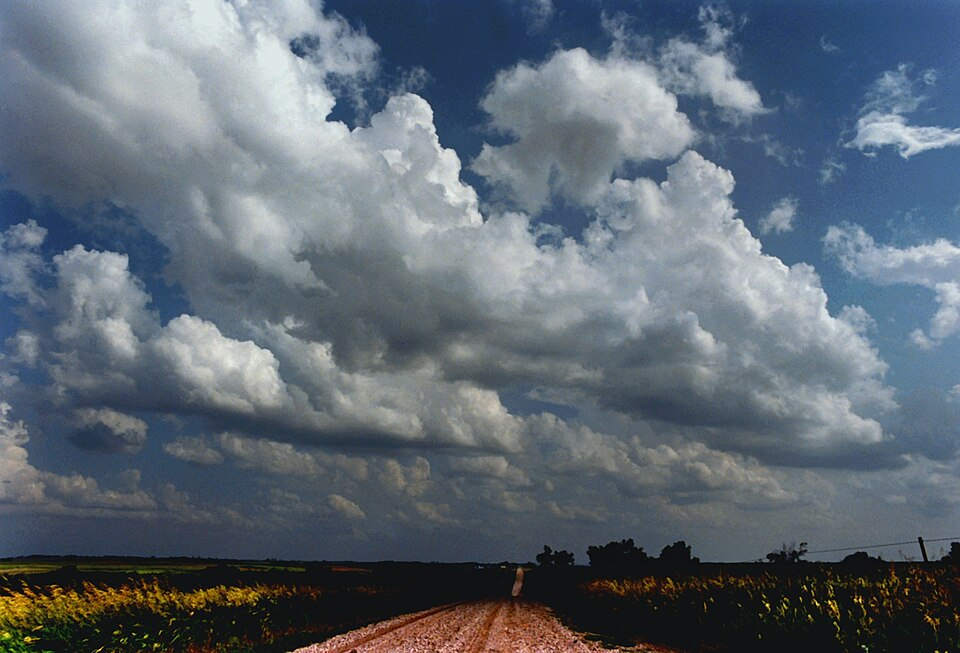
\includegraphics[width=\linewidth]{images/book1/g4-cumulus.jpg}

{\small \omterm{def:g4:clouds-rain-snow:cloud-families}{Cumulus}, stapelwolken met een platte onderkant.}
\end{minipage}\hfill
\begin{minipage}[b]{0.49\linewidth}\centering
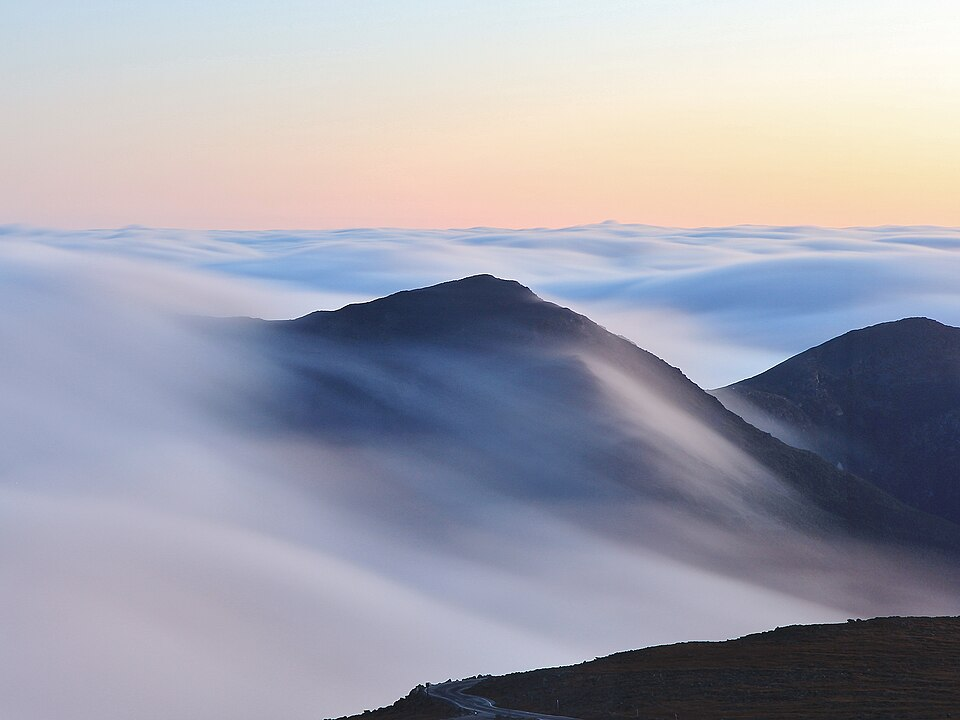
\includegraphics[width=\linewidth]{images/book1/g4-stratus.jpg}

{\small \omterm{def:g4:clouds-rain-snow:cloud-families}{Stratus}: een vlakke laag, hier van bovenaf gezien, vanaf een \omterm{def:g1:landscapes-around-us:landform}{berg}.}
\end{minipage}

\medskip
\begin{minipage}[b]{0.49\linewidth}\centering
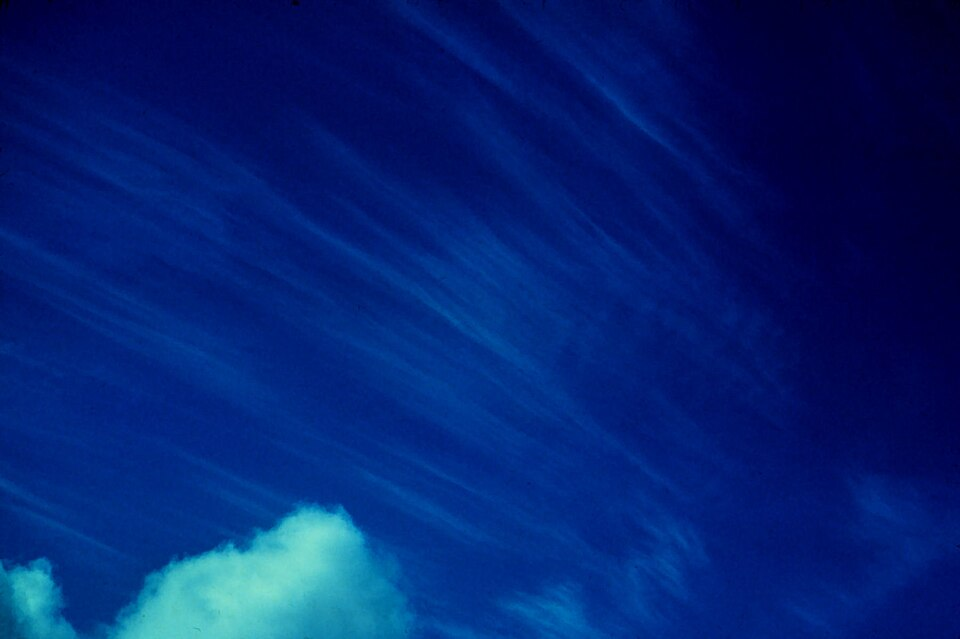
\includegraphics[width=\linewidth]{images/book1/g4-cirrus.jpg}

{\small \omterm{def:g4:clouds-rain-snow:cloud-families}{Cirrus}: dunne draden van ijs, heel hoog (met onderaan een kleine \omterm{def:g4:clouds-rain-snow:cloud-families}{cumulus}).}
\end{minipage}\hfill
\begin{minipage}[b]{0.49\linewidth}\centering
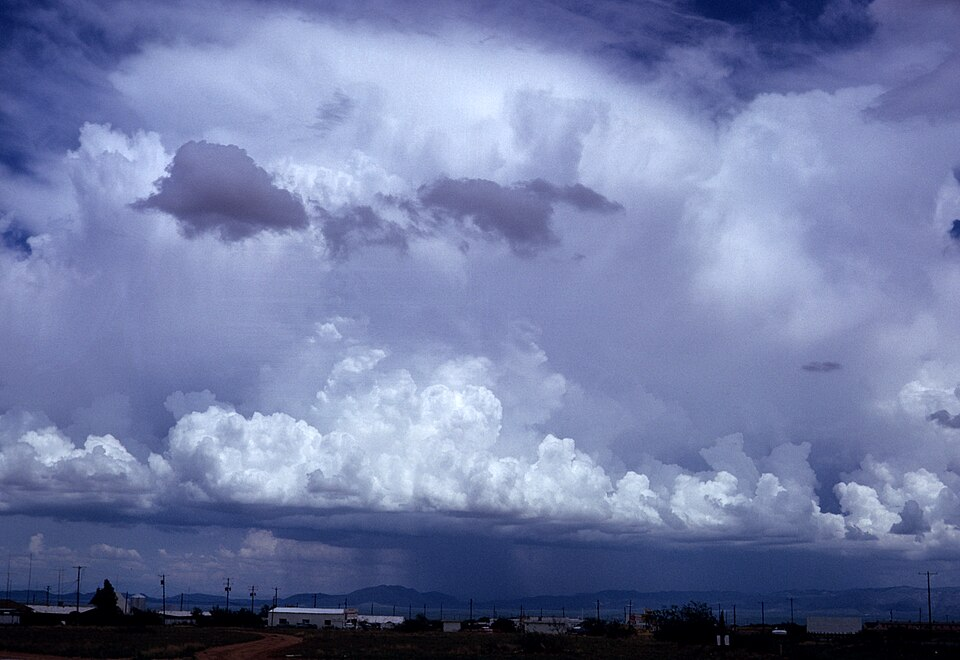
\includegraphics[width=\linewidth]{images/book1/g4-cumulonimbus.jpg}

{\small Een \omterm{def:g4:clouds-rain-snow:cloud-families}{cumulonimbus}: een toren van \omterm{def:g4:clouds-rain-snow:cloud}{wolken}; uit zijn donkere onderkant valt \omterm{def:g4:clouds-rain-snow:precipitation}{regen}.}
\end{minipage}

\smallskip
{\small Foto's: NOAA Photo Library (publiek domein): S. Corfidi
(\omterm{def:g4:clouds-rain-snow:cloud-families}{cumulus}), R. F. Kresge (\omterm{def:g4:clouds-rain-snow:cloud-families}{cirrus}), collectie B. Hooke (\omterm{def:g4:clouds-rain-snow:cloud-families}{cumulonimbus}).}
% ledger: noaa:photos-g4
\label{fig:g4:clouds-rain-snow:photos}
\end{omfigure}

Hoe hoog zweven \omterm{def:g4:clouds-rain-snow:cloud}{wolken}? Dat hangt af van de familie. Lage \omterm{def:g4:clouds-rain-snow:cloud}{wolken}, zoals
\omterm{def:g4:clouds-rain-snow:cloud-families}{stratus} en de onderkant van \omterm{def:g4:clouds-rain-snow:cloud-families}{cumulus}, zweven van vlak boven de grond tot
ongeveer 2 kilometer hoog. \omterm{def:g4:clouds-rain-snow:cloud-families}{Cirrus} zweven heel hoog, buiten de tropen en de
poolgebieden tussen ongeveer 5 en 13 kilometer --- vaak hoger dan de
hoogste \omterm{def:g1:landscapes-around-us:landform}{berg} op Aarde. Een \omterm{def:g4:clouds-rain-snow:cloud-families}{cumulonimbus} reikt helemaal van een lage
onderkant tot de bovenkant van de wolkenlagen.
% ledger: wmo:cloud-levels, wmo:cumulonimbus

\begin{omfigure}
\begin{tikzpicture}[x=1cm, y=0.5cm, font=\small]
  % height scale
  \draw[black!60] (0,0) -- (0,14);
  \foreach \h in {0,2,...,14} {
    \draw[black!60] (-0.1,\h) -- (0,\h);
    \node[anchor=east, font=\scriptsize] at (-0.12,\h) {\h\,km};
  }
  \node[anchor=south, font=\scriptsize, align=center] at (0,14.2) {hoogte};
  % ground and a mountain for comparison
  \fill[green!35!black!50] (0.2,0) -- (11.4,0) -- (11.4,-0.4) -- (0.2,-0.4) -- cycle;
  \fill[black!35] (8.6,0) -- (9.9,8.8) -- (10.2,8.4) -- (11.2,0) -- cycle;
  \fill[white, draw=black!45, line width=0.3pt] (9.65,7.2) -- (9.9,8.8) -- (10.2,8.4) -- (10.4,7.0) -- (10.1,7.4) -- (9.9,7.0) -- cycle;
  \node[font=\scriptsize, align=center] at (9.9,10.2) {de hoogste\\berg};
  % levels
  \fill[blue!6] (0.2,0.15) rectangle (8.3,2);
  \fill[blue!10] (0.2,5) rectangle (8.3,13);
  \node[anchor=west, font=\scriptsize, text=blue!50!black] at (0.3,1.65) {lage wolken};
  \node[anchor=west, font=\scriptsize, text=blue!50!black] at (0.3,12.6) {hoge wolken};
  % stratus: a flat grey layer
  \fill[black!25, rounded corners=2pt] (0.6,0.6) rectangle (2.6,1.3);
  \node[font=\scriptsize] at (1.6,-1.1) {stratus};
  % cumulus
  \pic[scale=0.7, transform shape] at (4.0,0.9) {puffycloud};
  \node[font=\scriptsize] at (4.0,-1.1) {cumulus};
  % cirrus: wisps
  \foreach \y in {9.4,10.0,10.6} {
    \draw[black!50, line width=0.6pt] (0.8,\y) .. controls (1.4,\y+0.5) and (2.0,\y+0.1) .. (2.6,\y+0.6);
  }
  \node[font=\scriptsize] at (1.7,8.5) {cirrus};
  % cumulonimbus: tower with an anvil
  \fill[black!15, draw=black!45, line width=0.4pt]
    (5.4,1.0) .. controls (5.2,4) and (5.6,8) .. (5.9,11.2)
    .. controls (5.0,11.6) and (4.6,12.0) .. (4.8,12.3)
    -- (8.1,12.3) .. controls (8.2,12.0) and (7.8,11.6) .. (7.0,11.2)
    .. controls (7.3,8) and (7.6,4) .. (7.4,1.0) -- cycle;
  \fill[black!45] (5.4,1.0) rectangle (7.4,1.4);
  \foreach \x in {5.7,6.1,6.5,6.9,7.2}
    \draw[omWxRain, line width=0.6pt] (\x,0.95) -- (\x-0.15,0.15);
  \node[font=\scriptsize] at (6.4,-1.1) {cumulonimbus};
\end{tikzpicture}

{\small Hoe hoog de vier wolkenfamilies zweven (hoogten in kilometer, voor
gebieden die niet tropisch en niet polair zijn). \omterm{def:g4:clouds-rain-snow:cloud-families}{Stratus} en de onderkant
van \omterm{def:g4:clouds-rain-snow:cloud-families}{cumulus} zijn laag; \omterm{def:g4:clouds-rain-snow:cloud-families}{cirrus} zijn vaak hoger dan de hoogste \omterm{def:g1:landscapes-around-us:landform}{berg}. Een
\omterm{def:g4:clouds-rain-snow:cloud-families}{cumulonimbus} reikt van een lage onderkant tot de bovenkant van de
wolkenlagen. Hoogten naar de wolkenatlas van de
Wereld Meteorologische Organisatie.}
\label{fig:g4:clouds-rain-snow:heights}
% ledger: wmo:cloud-levels, tht:everest
\end{omfigure}

\begin{method}[Een wolk benoemen]\label{met:g4:clouds-rain-snow:naming}
Kijk naar de hemel en stel drie vragen:
\begin{enumerate}
  \item Is het een hoop met een platte onderkant? Dan is het een \omterm{def:g4:clouds-rain-snow:cloud-families}{cumulus}
        --- en als hij oprijst tot een enorme donkere toren, een
        \omterm{def:g4:clouds-rain-snow:cloud-families}{cumulonimbus}.
  \item Is het een vlak, egaal dek dat de hele hemel verbergt? Dan is het
        een \omterm{def:g4:clouds-rain-snow:cloud-families}{stratus}.
  \item Bestaat hij uit dunne witte draden, heel hoog? Dan is het een \omterm{def:g4:clouds-rain-snow:cloud-families}{cirrus}.
\end{enumerate}
\end{method}

\begin{remark}[Wolken vertellen het weer]\label{rem:g4:clouds-rain-snow:tell}
Kleine \omterm{def:g4:clouds-rain-snow:cloud-families}{cumulus} in een blauwe hemel betekenen mooi \omterm{def:g1:watching-the-weather:weather}{weer}. Een grijze \omterm{def:g4:clouds-rain-snow:cloud-families}{stratus}
brengt een sombere dag, soms met motregen. Een \omterm{def:g4:clouds-rain-snow:cloud-families}{cumulonimbus} brengt een
korte, hevige bui, vaak met donder, bliksem en windvlagen --- soms met
\omterm{def:g4:clouds-rain-snow:precipitation}{hagel}. \omterm{def:g4:clouds-rain-snow:cloud-families}{Cirrus} brengen geen \omterm{def:g4:clouds-rain-snow:precipitation}{regen}, maar als ze zich uitbreiden en dikker
worden, volgt er vaak een dag later \omterm{def:g4:clouds-rain-snow:precipitation}{regen}.
\end{remark}

\section{Regen, sneeuw en hagel}

In een \omterm{def:g4:clouds-rain-snow:cloud}{wolk} botsen de piepkleine druppeltjes tegen elkaar en smelten ze
samen, of groeien ijskristallen ten koste van de druppeltjes. Een
wolkendruppel of een kristal dat groot en zwaar genoeg is geworden, kan
niet meer zweven: hij valt.

\begin{definition}[Neerslag]\label{def:g4:clouds-rain-snow:precipitation}
\emph{Neerslag}\index{neerslag} is water dat uit een \omterm{def:g4:clouds-rain-snow:cloud}{wolk} naar de grond
valt: \emph{regen}\index{regen} (druppels vloeibaar water),
\emph{sneeuw}\index{sneeuw} (vlokken van aan elkaar geplakte ijskristallen)
of \emph{hagel}\index{hagel} (balletjes ijs, hagelstenen genoemd, die uit
onweerswolken vallen).
\end{definition}

Of het regent of sneeuwt, hangt af van de temperatuur van de lucht waar de
\omterm{def:g4:clouds-rain-snow:precipitation}{neerslag} doorheen valt. Sneeuwvlokken ontstaan hoog in de koude \omterm{def:g4:clouds-rain-snow:cloud}{wolk}. Is de
lucht eronder lang genoeg warmer dan \SI{0}{\celsius}, dan smelten ze
onderweg en bereiken ze ons als \omterm{def:g4:clouds-rain-snow:precipitation}{regen}. Vriest het helemaal tot aan de grond,
dan komen ze aan als \omterm{def:g4:clouds-rain-snow:precipitation}{sneeuw}.

\begin{omfigure}

\includegraphics[width=0.55\linewidth]{images/book1/ai/g4-snowflakes.jpg}

{\small Kinderen vangen sneeuwvlokken op een donkere handschoen: elke vlok
bestaat uit ijskristallen.}
\end{omfigure}

\omterm{def:g4:clouds-rain-snow:precipitation}{Hagel} valt alleen uit \omterm{def:g4:clouds-rain-snow:cloud-families}{cumulonimbus}. In de toren voeren sterke opwaartse
winden ijskorrels verschillende keren op en neer; bij elke tocht komt er
een nieuw laagje ijs bij, zoals de lagen van een ui, tot de hagelsteen te
zwaar is om door de wind gedragen te worden.

\begin{omfigure}
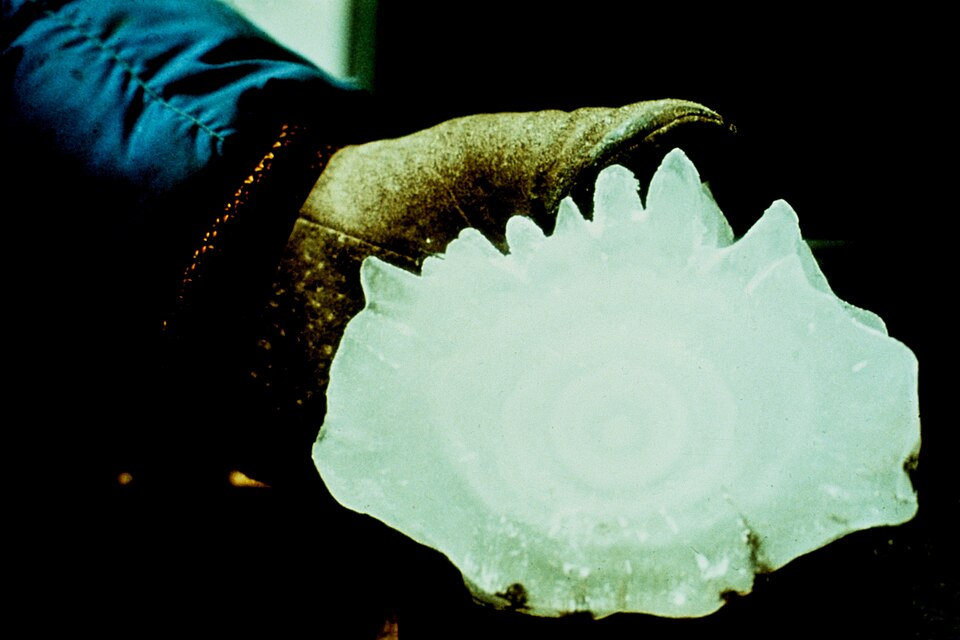
\includegraphics[width=0.5\linewidth]{images/book1/g4-hailstone.jpg}

{\small Een heel grote hagelsteen in een hand met een handschoen. De ringen
laten de lagen ijs zien die hij in de onweerswolk heeft verzameld. Foto:
NOAA Photo Library (publiek domein).}
% ledger: noaa:photos-g4
\end{omfigure}

\section{Het weer meten}

Om te zeggen hoeveel het regende, hoe warm het was of waar de wind vandaan
kwam, zijn woorden niet genoeg: we hebben instrumenten nodig, en getallen.

\begin{definition}[Regenmeter]\label{def:g4:clouds-rain-snow:rain-gauge}
Een \emph{regenmeter}\index{regenmeter} is een bak die de \omterm{def:g4:clouds-rain-snow:precipitation}{regen} opvangt die
op zijn opening valt. De hoogte van het opgevangen water wordt gemeten in
millimeter: ``5 millimeter \omterm{def:g4:clouds-rain-snow:precipitation}{regen}'' betekent dat de \omterm{def:g4:clouds-rain-snow:precipitation}{regen} op vlakke grond
een laagje water van 5 millimeter dik zou hebben gemaakt, als er niets van
was weggestroomd of in de grond was gezakt.
\end{definition}

\begin{remark}[Een millimeter regen is veel water]\label{rem:g4:clouds-rain-snow:litre}
Een millimeter \omterm{def:g4:clouds-rain-snow:precipitation}{regen} lijkt piepklein in de \omterm{def:g4:clouds-rain-snow:rain-gauge}{regenmeter}. Maar op een stuk
grond van één meter bij één meter is het één liter water: een grote fles.
Op een schoolplein van duizend vierkante meter brengt een regenbui van
10 millimeter tienduizend liter: genoeg om duizend emmers van elk 10 liter
te vullen.
\end{remark}

\begin{omfigure}
\begin{tikzpicture}[font=\small]
  % funnel
  \draw[black!70, line width=0.8pt] (-1.2,6.6) -- (-0.35,5.8) -- (-0.35,5.4);
  \draw[black!70, line width=0.8pt] (1.2,6.6) -- (0.35,5.8) -- (0.35,5.4);
  \draw[black!70, line width=0.8pt] (-1.2,6.6) -- (1.2,6.6);
  % tube
  \fill[blue!25] (-0.45,0) rectangle (0.45,2.4);
  \draw[black!70, line width=0.8pt] (-0.45,5.4) -- (-0.45,0) -- (0.45,0) -- (0.45,5.4);
  \foreach \m in {0,1,...,50} {
    \pgfmathsetmacro{\yy}{\m*0.1}
    \draw[black!60] (0.45,\yy) -- ++(-0.12,0);
  }
  \foreach \m in {0,5,10,...,50} {
    \pgfmathsetmacro{\yy}{\m*0.1}
    \draw[black!80] (0.45,\yy) -- ++(-0.25,0);
    \node[anchor=west, font=\scriptsize] at (0.5,\yy) {\m};
  }
  \node[anchor=west, font=\scriptsize] at (1.0,5.0) {mm};
  % reading line
  \draw[red!70!black, -{Stealth}] (-1.6,2.4) -- (-0.5,2.4);
  \node[anchor=east, align=right, font=\scriptsize] at (-1.65,2.4) {lees het\\niveau hier af};
  \node[anchor=west, font=\scriptsize] at (1.9,2.4) {$\leftarrow$ 24\,mm regen};
\end{tikzpicture}

{\small Een eenvoudige \omterm{def:g4:clouds-rain-snow:rain-gauge}{regenmeter}: een trechter vangt de \omterm{def:g4:clouds-rain-snow:precipitation}{regen} op en een
buis met een millimeterschaal houdt hem vast. Lees het waterniveau af met
je oog op dezelfde hoogte. Hier is er 24 millimeter gevallen sinds de
\omterm{def:g4:clouds-rain-snow:rain-gauge}{regenmeter} het laatst werd geleegd.}
\label{fig:g4:clouds-rain-snow:gauge}
\end{omfigure}


\begin{definition}[Windvaan]\label{def:g4:clouds-rain-snow:wind-vane}
Een \emph{windvaan}\index{windvaan} is een pijl die vrij draait op een
mast. De wind duwt tegen zijn staart, zodat de pijl altijd wijst naar de
richting waar de wind \emph{vandaan} komt.
\end{definition}

\begin{definition}[Weerstation]\label{def:g4:clouds-rain-snow:weather-station}
Een \emph{weerstation}\index{weerstation} is een plek waar het \omterm{def:g1:watching-the-weather:weather}{weer} elke dag
wordt gemeten, altijd op dezelfde manier, met instrumenten: een thermometer
in een geventileerde witte hut, een \omterm{def:g4:clouds-rain-snow:rain-gauge}{regenmeter} in het open veld, een
\omterm{def:g4:clouds-rain-snow:wind-vane}{windvaan} op een mast.
\end{definition}

De thermometer staat in de schaduw, in een witte hut met latjes aan de
zijkanten die de lucht doorlaten maar de zon en de \omterm{def:g4:clouds-rain-snow:precipitation}{regen} tegenhouden. Het
Met Office, de weerdienst van het Verenigd Koninkrijk, zet hem
\SI{1.25}{\metre} boven de grond. De \omterm{def:g4:clouds-rain-snow:rain-gauge}{regenmeter} staat in het open veld, ver
van muren en bomen die hem tegen de \omterm{def:g4:clouds-rain-snow:precipitation}{regen} zouden beschutten, met zijn
opening een beetje boven de grond. De \omterm{def:g4:clouds-rain-snow:wind-vane}{windvaan} staat hoog op zijn mast,
boven de obstakels die de wind zouden afbuigen.
% ledger: mo:screen-height, mo:raingauge

\begin{omfigure}
\begin{tikzpicture}[font=\small, x=1cm, y=1cm]
  % grass
  \fill[green!40!black!45] (-0.5,0) rectangle (11,-0.25);
  \foreach \x in {-0.3,0.1,...,10.8} \draw[green!45!black] (\x,0) -- ++(0.06,0.14);
  % screen on legs
  \draw[black!70, line width=1pt] (0.8,0) -- (0.8,1.25) (2.2,0) -- (2.2,1.25);
  \fill[white, draw=black!70] (0.6,1.25) rectangle (2.4,2.4);
  \foreach \y in {1.4,1.55,...,2.25} \draw[black!40] (0.7,\y) -- (2.3,\y-0.08);
  \fill[white, draw=black!70] (0.45,2.4) -- (1.5,2.75) -- (2.55,2.4) -- cycle;
  \draw[black!60, <->] (2.8,0) -- node[right, font=\scriptsize, align=left] {ongeveer\\1.25\,m} (2.8,1.25);
  \node[align=center, font=\scriptsize] at (1.5,3.25) {thermometer in een\\witte hut met latjes};
  % rain gauge
  \fill[black!15, draw=black!70] (5.4,0) rectangle (5.9,0.4);
  \draw[black!70] (5.3,0.55) -- (5.4,0.4) (6.0,0.55) -- (5.9,0.4);
  \node[align=center, font=\scriptsize] at (5.65,1.2) {regenmeter,\\in het open veld};
  % tree far away
  \fill[brown!60!black] (7.3,0) rectangle (7.5,1.3);
  \fill[green!50!black!70] (7.4,2.1) circle (0.85);
  % wind vane on a mast
  \draw[black!70, line width=1pt] (9.8,0) -- (9.8,4.2);
  \draw[black!80, line width=1.4pt, -{Latex[length=3mm]}] (10.6,4.4) -- (9.0,4.4);
  \fill[black!80] (10.6,4.4) -- (10.9,4.65) -- (10.9,4.15) -- cycle;
  \node[align=center, font=\scriptsize] at (9.8,5.05) {windvaan op een hoge mast};
  \node[anchor=west, font=\scriptsize, align=left] at (10.1,3.4) {wijst waar de\\wind vandaan komt};
\end{tikzpicture}

{\small Een klein \omterm{def:g4:clouds-rain-snow:weather-station}{weerstation}. De thermometer staat in de schaduw, in een
witte hut met latjes, ongeveer 1.25 meter boven het gras; de \omterm{def:g4:clouds-rain-snow:rain-gauge}{regenmeter}
staat in het open veld, ver van de boom; de \omterm{def:g4:clouds-rain-snow:wind-vane}{windvaan} staat hoog boven de
obstakels.}
\label{fig:g4:clouds-rain-snow:station}
% ledger: mo:screen-height
\end{omfigure}

\begin{inthefield}[Een weerstation op het schoolplein]
Veel scholen hebben een klein \omterm{def:g4:clouds-rain-snow:weather-station}{weerstation} in een hoek van het schoolplein.
Elke ochtend op hetzelfde tijdstip lezen twee leerlingen de thermometer af,
lezen de \omterm{def:g4:clouds-rain-snow:rain-gauge}{regenmeter} af en maken hem leeg, en noteren waar de \omterm{def:g4:clouds-rain-snow:wind-vane}{windvaan} heen
wijst. Zo bouwt de klas week na week een verslag op van haar eigen weer.
\end{inthefield}

\begin{omfigure}
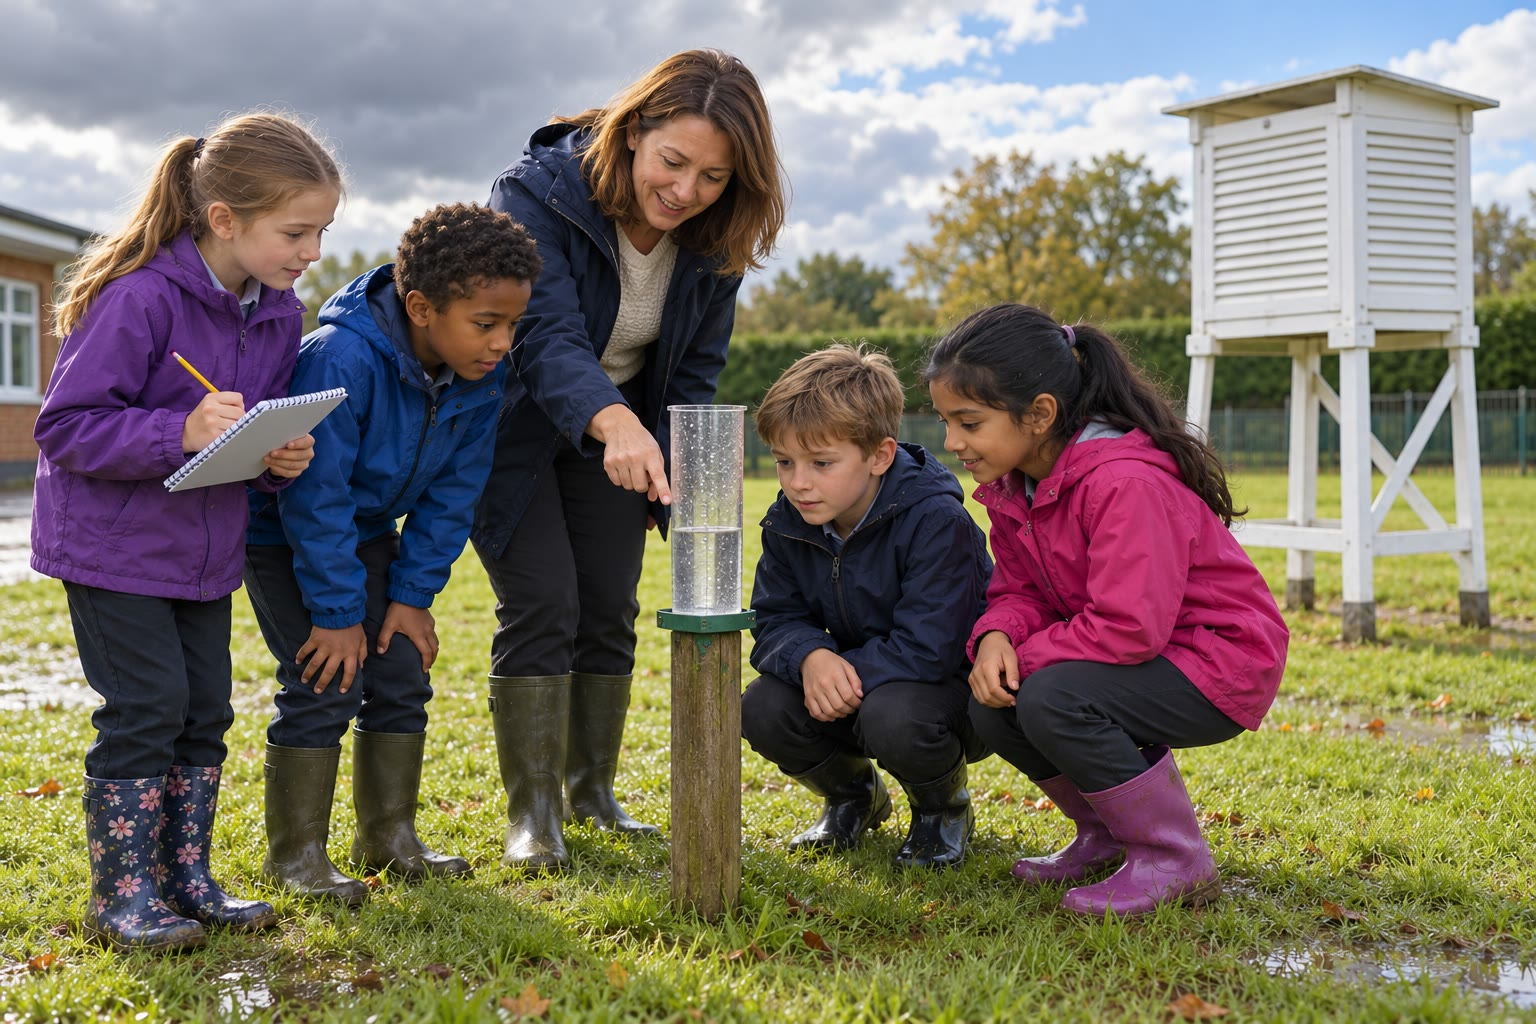
\includegraphics[width=0.55\linewidth]{images/book1/ai/g4-rain-gauge-class.jpg}

{\small Leerlingen lezen de \omterm{def:g4:clouds-rain-snow:rain-gauge}{regenmeter} op het schoolplein af.}
\end{omfigure}

\begin{method}[Een staafdiagram van de regen tekenen]\label{met:g4:clouds-rain-snow:bar-chart}
Zo teken je de \omterm{def:g4:clouds-rain-snow:precipitation}{regen} van een week:
\begin{enumerate}
  \item teken een horizontale lijn en schrijf de dagen eronder, op gelijke
        afstanden;
  \item teken links een verticale lijn en zet er millimeters bij, in
        gelijke stappen (bijvoorbeeld om de 2 millimeter);
  \item teken boven elke dag een staaf die zo hoog is als de \omterm{def:g4:clouds-rain-snow:precipitation}{regen} van die
        dag; een dag zonder \omterm{def:g4:clouds-rain-snow:precipitation}{regen} krijgt helemaal geen staaf;
  \item geef de grafiek een titel en schrijf de eenheid, mm, bij de
        verticale lijn.
\end{enumerate}
\end{method}

\begin{example}[Een week regen op school]\label{ex:g4:clouds-rain-snow:week}
De klas las een week lang elke ochtend de \omterm{def:g4:clouds-rain-snow:rain-gauge}{regenmeter} af en vond: maandag 0,
dinsdag 4, woensdag 12, donderdag 7, vrijdag 0, zaterdag 2, zondag
5 millimeter. De natste dag was woensdag. Op maandag en op vrijdag regende
het niet. In de hele week viel er $0 + 4 + 12 + 7 + 0 + 2 + 5 = 30$
millimeter. Woensdag alleen bracht 12 van de 30 millimeter, dat is
$\frac{12}{30} = \frac{2}{5}$ van de \omterm{def:g4:clouds-rain-snow:precipitation}{regen} van de week.
\end{example}

\begin{omfigure}
\begin{tikzpicture}
\begin{axis}[ybar, bar width=14pt, width=0.8\linewidth, height=5.4cm,
    ymin=0, ymax=14, ytick={0,2,...,14}, ylabel={regen (mm)},
    symbolic x coords={Mon,Tue,Wed,Thu,Fri,Sat,Sun}, xtick=data, xticklabels={ma,di,wo,do,vr,za,zo},
    axis x line*=bottom, axis y line*=left, ymajorgrids, grid style={gray!25},
    nodes near coords, nodes near coords style={font=\scriptsize},
    every axis label/.append style={font=\small}, tick label style={font=\small},
    title={Regen op school, één week}, title style={font=\small}]
  \addplot[fill=omWxRain!70, draw=omWxRain!60!black] coordinates
    {(Mon,0) (Tue,4) (Wed,12) (Thu,7) (Fri,0) (Sat,2) (Sun,5)};
\end{axis}
\end{tikzpicture}

{\small De week van \cref{ex:g4:clouds-rain-snow:week} als staafdiagram.}
\label{fig:g4:clouds-rain-snow:bars}
\end{omfigure}

\section{Oefeningen}

\begin{exercise}[$\star$]\label{exo:g4:clouds-rain-snow:1}
Waaruit bestaat een \omterm{def:g4:clouds-rain-snow:cloud}{wolk}? Wat is \omterm{def:g4:clouds-rain-snow:cloud}{mist}?
\end{exercise}

\begin{exercise}[$\star$]\label{exo:g4:clouds-rain-snow:2}
Benoem de \omterm{def:g4:clouds-rain-snow:cloud}{wolk}: (a) een vlak grijs dek dat de hele hemel verbergt; (b) dunne
witte draden heel hoog in een blauwe hemel; (c) witte hopen met een platte
onderkant, als watjes; (d) een enorme donkere toren met een platte top, die
onweer brengt.
\end{exercise}

\begin{exercise}[$\star$]\label{exo:g4:clouds-rain-snow:3}
\omterm{def:g4:clouds-rain-snow:precipitation}{Regen}, \omterm{def:g4:clouds-rain-snow:precipitation}{sneeuw} of \omterm{def:g4:clouds-rain-snow:precipitation}{hagel}? (a) balletjes ijs die uit een onweerswolk vallen;
(b) druppels vloeibaar water; (c) vlokken van ijskristallen.
\end{exercise}

\begin{exercise}[$\star$]\label{exo:g4:clouds-rain-snow:4}
Welk instrument meet: (a) de \omterm{def:g4:clouds-rain-snow:precipitation}{regen}; (b) de temperatuur; (c) waar de wind
vandaan komt?
\end{exercise}

\begin{exercise}[$\star$]\label{exo:g4:clouds-rain-snow:5}
In de \omterm{def:g4:clouds-rain-snow:rain-gauge}{regenmeter} die op pagina~\pageref{fig:g4:clouds-rain-snow:gauge} is
getekend, komt het water nu tot het streepje 17. Hoeveel millimeter \omterm{def:g4:clouds-rain-snow:precipitation}{regen}
is er gevallen? Hoeveel millimeter erbij zou het tot 20 brengen?
\end{exercise}

\begin{exercise}[$\star$]\label{exo:g4:clouds-rain-snow:6}
Kijk naar het staafdiagram op pagina~\pageref{fig:g4:clouds-rain-snow:bars}.
Welke dag was de natste? Op welke dagen regende het niet? Op welke dag viel
er 7 millimeter?
\end{exercise}

\begin{exercise}[$\star\star$]\label{exo:g4:clouds-rain-snow:7}
Op de ochtend van een sneeuwdag komen de sneeuwvlokken in het bergdorp tot
op de grond, maar in het \omterm{def:g1:landscapes-around-us:landform}{dal} eronder regent het. Leg het verschil uit met
behulp van de temperatuur van de lucht.
\end{exercise}

\begin{exercise}[$\star\star$]\label{exo:g4:clouds-rain-snow:8}
Een andere week vindt de klas: maandag 3, dinsdag 0, woensdag 1, donderdag
9, vrijdag 6, zaterdag 0, zondag 1 millimeter. Teken het staafdiagram.
Hoeveel millimeter viel er in de week? Welk deel van de \omterm{def:g4:clouds-rain-snow:precipitation}{regen} van de week
viel op donderdag?
\end{exercise}

\begin{exercise}[$\star\star$]\label{exo:g4:clouds-rain-snow:9}
Waarom moet de \omterm{def:g4:clouds-rain-snow:rain-gauge}{regenmeter} in het open veld staan, ver van muren en bomen?
Waarom staat de thermometer in een witte hut in de schaduw, en niet in de
volle zon?
\end{exercise}

\begin{exercise}[$\star\star$]\label{exo:g4:clouds-rain-snow:10}
De \omterm{def:g4:clouds-rain-snow:wind-vane}{windvaan} wijst naar het westen. Waar komt de wind vandaan? Waar gaat hij
heen?
\end{exercise}

\begin{exercise}[$\star\star\star$]\label{exo:g4:clouds-rain-snow:11}
Op een schoolplein van 500 vierkante meter valt 8 millimeter \omterm{def:g4:clouds-rain-snow:precipitation}{regen}. Hoeveel
liter water viel er op het schoolplein? Gebruik
\cref{rem:g4:clouds-rain-snow:litre}. Een gieter bevat 10 liter: hoeveel
gieters is dat?
\end{exercise}
